


\subsection{Conceptual predictions for DLT and Surprisal Theory}

\begin{figure}
    \centering
	\begin{tabular}{cccc}
		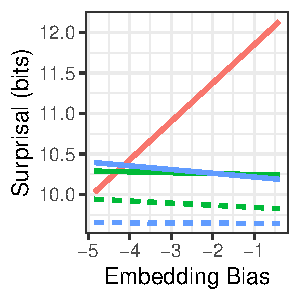
\includegraphics[width=0.2\textwidth]{figures/predictions-surprisal-zero_VN_GPT2XL_Bits.pdf} 
	\end{tabular}
	\caption{Surprisal computed from fully veridical context representations (corresponding to $\delta=20$) as computed by GPT-2-XL, the largest version of GPT-2. Compare Figure 3 (right, Surprisal Theory) in the main paper for corresponding results from GPT-2-Medium.}
    \label{fig:zero-noise}
\end{figure}



To derive conceptual predictions from DLT, we computed Integration Cost on the last verb. This depends on the number of discourse referents between the last verb and the first noun, which is 0 in the One condition, 2 or 3 (depending on the precise sentences, e.g., 3 in \textit{the report that the \textbf{doctor} \textbf{cured} the \textbf{patient}}) in the Two condition, and 4 or 5 (depending on the precise sentences, e.g., 5 in \textit{the report that the \textbf{doctor} who the \textbf{senator} \textbf{admired} \textbf{cured} the \textbf{patient}}) in the Three condition.

This qualitative prediction is shared by memory-based models more broadly, as they fundamentally predict that dependencies are harder to resolve when more material intervenes  \citep{mcelree2000sentence,mcelree-memory-2003,lewis2005activation}.
Models also make specific predictions about how this cost is modulated, in particular due to similarity-based interference, but this does not predict effects related to Embedding Bias (see Section~\ref{sec:surface-strings}).
On a conceptual level, models in the cue-based retrieval paradigm may potentially predict an effect of semantic compatibility (see Section~\ref{sec:surface-strings}), but this does not arise in computationally explicit models in in this paradigm \citep{lewis2005activation,Rasmussen2018LeftCornerPW,Dotlacil2020Parsing}.\footnote{We are grateful to Jakub Dotla{\v c}il for help with running the model from \citet{Dotlacil2020Parsing}.}


For Surprisal Theory, we first noted that, when embedding bias is very high, the chance that a noun is followed immediately by a verb has to be relatively low.
We thus predicted a positive main effect of embedding bias on surprisal of the last verb in the \textsc{One} condition.
On the other hand, in the \textsc{Two} and \textsc{Three} condition, after observing a clause, we do not expect that the chance of observing another verb depends on either embedding bias of semantic compatibility.
To the extent that Surprisal Theory may predict a difference between the \textsc{Two} and \textsc{Three} conditions, it would be in the \emph{opposite} direction of the empirically observed one (lower surprisal in the \textsc{Three} condition), as additional intervening material should make prediction of the final verb easier.
These conceptual predictions are in agreement with the surprisals computed both by GPT-2 Medium as reported in the main paper, and by GPT-2 XL, the strongest model in the GPT-2 family, at zero noise (Figure~\ref{fig:zero-noise}).
Note that the effect of compatibility is numerically even in the opposite direction compared to Resource-Rational Lossy-Context Surprisal and human reading times. 

\subsection{Implications for Cue-Based Retrieval Accounts of Center Embedding Difficulty}\label{sec:surface-strings}


The difficulty patterns observed in our experiments are distinct from the predictions of existing theories of sentence processing.
The findings thus pose an interesting challenge for previous, more mechanistic models of sentence processing, constraining the search for future models that could account for our findings within those modeling frameworks.
Here, we discuss prospects and challenges for accounting for our experimental results within a prominent family of previous approaches based on a left-corner parser using associative retrieval as proposed by \citet{lewis2005activation} (similarly \citet{Rasmussen2018LeftCornerPW, Dotlacil2020Parsing}).


In the literature on cue-based retrieval, the difficulty of center embeddings arises because syntactic structures are established not using order information (as in a stack), but using associative retrieval of content-addressable memory structures \citep{mcelree-memory-2003,lewis2005activation,parker2017cue}.
When encountering the second-to-last verb in a center embedding structure, humans may erroneously retrieve the wrong noun as the subject of this verb, leaving the final verb stranded \citep{mcelree-memory-2003,lewis2005activation,Haussler2015AnIA}.
Conceptually, this idea is closely related to our model, where processing is disrupted when the information retrieved from short-term memory suggests  attaching the second verb to the first noun with relatively high posterior probability.
\citet{lewis2005activation} describe a computationally implemented model of sentence comprehension that also includes an account of the difficulty of center embeddings.
In this model, retrieval failure frequently occurs at the last verb because the prediction of a main clause verb was retrieved too early, leaving it unavailable when the final verb is encountered \citep[p. 406]{lewis2005activation}.\footnote{While their model as implemented did not actually show retrieval failure in the structures corresponding to our \textsc{Three} condition (SC/RC in their terminology) (they do not report results for the \textsc{Two} condition), we believe that the parser rules in their model could be adapted to produce it in the model predictions. }

In order to account for our empirical results, such models thus need to be extended to predict in detail when the correct noun is more or less likely to be retrieved as the subject of the second-to-last verb.
Two effects need to be accounted for specifically, namely the effects of semantic compatibility and of embedding bias in the \textsc{Two} and \textsc{Three} conditions.

An account of the effect of semantic compatibility seems relatively straightforward to implement within extensions of such models.
On an informal level (without formalization or computational implementation), \citet{Haussler2015AnIA} propose a \emph{Discrimination Hypothesis}, which states that integration of new material is disrupted when a clause intervenes after the correct integration site and ``an incorrect but similar integration site competes for attachment.''
To account for the difficulty of doubly-nested center embeddings (such as our \textsc{Three} condition), they propose that, when the second verb is encountered, the human parser erroneously retrieves the first (instead of the second) noun as the subject.
They also argue that the proposed Discrimination Hypothesis accounts for previous observations on the role of semantic properties of the second verb phrase \citep{gibson1999memory}, related to the effect of the Compatibility manipulation in our experiments. 
In Figure~\ref{fig:retrieval}A, we show the syntactic structure assigned to a stimulus in the \textsc{Two} condition in the grammatical formalism assumed by \citet{lewis2005activation}, based on X-Bar syntax \citep{Jackendoff1980XSA}.
Figure~\ref{fig:retrieval}B (left) illustrates the state of the parser before the word ``annoyed'' is received; each constituent in the syntactic tree is represented by a feature structure stored as a chunk in short-term memory (formalized in the ACTR-R framework, \citet{Anderson1990adaptive}), including information about syntactic categories, lexical items, and which other chunks a chunk is linked to in the syntactic tree.
The current tree has two open predictions that both require a finite verb, each represented by a chunk stored in memory.
As the parser relies on associative retrieval, and does not represent linear order, it needs to rely on other cues to identify which of the two nodes to attach ``annoyed'' to.
In this case, both subjects are semantically compatible with the verb, and the parser may (incorrectly) attach ``annoyed'' to $VP_1$. 
The parser then completes $VP_1$ and ends up believing that $IP_1$ is complete, leading to breakdown once ``was'' is observed (cf. \citet[][Section 6.3]{lewis2005activation}).
In contrast, when replacing ``annoyed'' with ``cured'', semantic cues strongly favor attaching ``annoyed'' to $VP_2$, avoiding prematurely declaring the sentence complete.
This mechanism could account for the effect of compatibility on reading times on the final verb; a full account would require a detailed specification of parser rules that percolate information about the subject through the tree and use it to determine attachment sites.



It is much less clear how the cue-based retrieval proposals might be extended to account for the effect of embedding bias: it is not obvious why embedding bias should determine how likely a noun is to be retrieved as the integration site for a subject-verb dependency, as embedding bias does not determine a noun's chance of being a subject.
One possibility is that the content of the chunks themselves is subject to loss, so that the CP node may be incorrectly recovered as a prepositional phrase node, depending on semantic and statistical cues.
Another possibility -- one we believe might be the most fruitful in searching for extensions of the  \citet{lewis2005activation}  model -- is that parser rules are sensitive to statistical patterns in the language.
The parser rules in the parser implemented by \citet{lewis2005activation} are not sensitive to the lexical difference between report/fact/..., but a rational parser with fine-grained awareness of the statistics of the language might well have such rules.
Indeed, given the fundamentally rational and adaptive nature of memory retrieval in the \citet{lewis2005activation} model, it is an appealing idea that memory retrieval should be impacted by the statistical structure of language and give rise to patterns resembling noisy-channel inferences. 
In a situation such as in Figure~\ref{fig:retrieval}B, a rational parser may have a specific rule stating -- for instance -- that, if there are two open VP predictions and one of them has as its subject a noun with very high embedding bias (such as ``fact''), a new verb should be preferentially attached to the other VP, as that is statistically likely to be inside a complement clause headed by that noun.
Such a rule would then prevent premature attachment to the top-level node.
Again, working out a full account would require specifying suitable parser rules, a nontrivial undertaking which may be an interesting problem for future work in the cue-based parsing paradigm.


We have seen that, generally speaking, the difficulty of center embeddings arises in associative retrieval-based parsing models because the parser makes choices based on local information available at the relevant chunks, ``guessing'' the next steps without a costly traversal of the full tree necessary to gain certainty about the correct next action \citep{mcelree-memory-2003,lewis2005activation,Haussler2015AnIA}.
The effect of words (e.g. ``that'') \emph{not being retained} in Resource-Rational Lossy-Context Surprisal corresponds to the effect of words and chunks (e.g., $CP_1$ in Figure~\ref{fig:retrieval}B) \emph{not being retrieved} when processing the next word in associative retrieval-based parsers.
We suggest that cases where the posterior $P(c|c')$ assigns \emph{high probability to structurally nonveridical variants} correspond to cases where parser rules make \emph{incorrect inferences about the structural position} of the next word by relying on a limited number of easily-retrieved chunks.
If the rules of a symbolic parser are rationally adapted to the statistics of the language, then the \emph{influence exerted by surface-similar variants on expectations} in lossy-context surprisal should correspond to rationally adaptated grammar rules \emph{attempting to infer the structural position of the next word based on limited information and the statistics of the language}.
Quite similarly to the low on-average surprisal achieved by resource-rational memory representations in our model, such heuristic choices based on local information may be rational on most sentences, but lead to breakdown in structures such as center embeddings.
We believe that these suggested correspondences may prove fruitful in searching for extensions of cue-based parsing models that can emulate the predictions of Resource-Rational Lossy-Context Surprisal.

A key difference between our proposed resource-rational model, and models of retrieval-based parsing such as that of \citet{lewis2005activation} is that the resource-rational objective function, coupled with the definition of lossy-context surprisal (Equation 1 in the main paper), and a specification of the average retention rate, are sufficient to derive model predictions on any input.
In contrast, for a retrieval-based parser, predictions are substantially dependent on the grammar and the parsing rules.
Whereas the effects observed in our experiments ``come for free'' under the resource-rational model, implementing them in a retrieval-based parser requires some, potentially arbitrary, decisions about grammar and parser rules.
We believe that identifying a rational modeling approach that could derive grammar and parsing rules in a principled manner is an interesting problem for future research, and might point the way towards models recapitulating the predictions of our resource-rational model within more mechanistic symbolic parsing models.
More generally, in agreement with \citet{parker2017cue}, we believe that finding cue-based retrieval models that are fully integrated with findings about probabilistic processing is an important open problem for psycholinguistic research. 
Such models could provide algorithmic-level counterparts to the computational-level model that we advance in this paper; the findings we describe constrain the search for such models.






\begin{figure}
    \centering
	\begin{tabular}{llll}
		(A) \\
		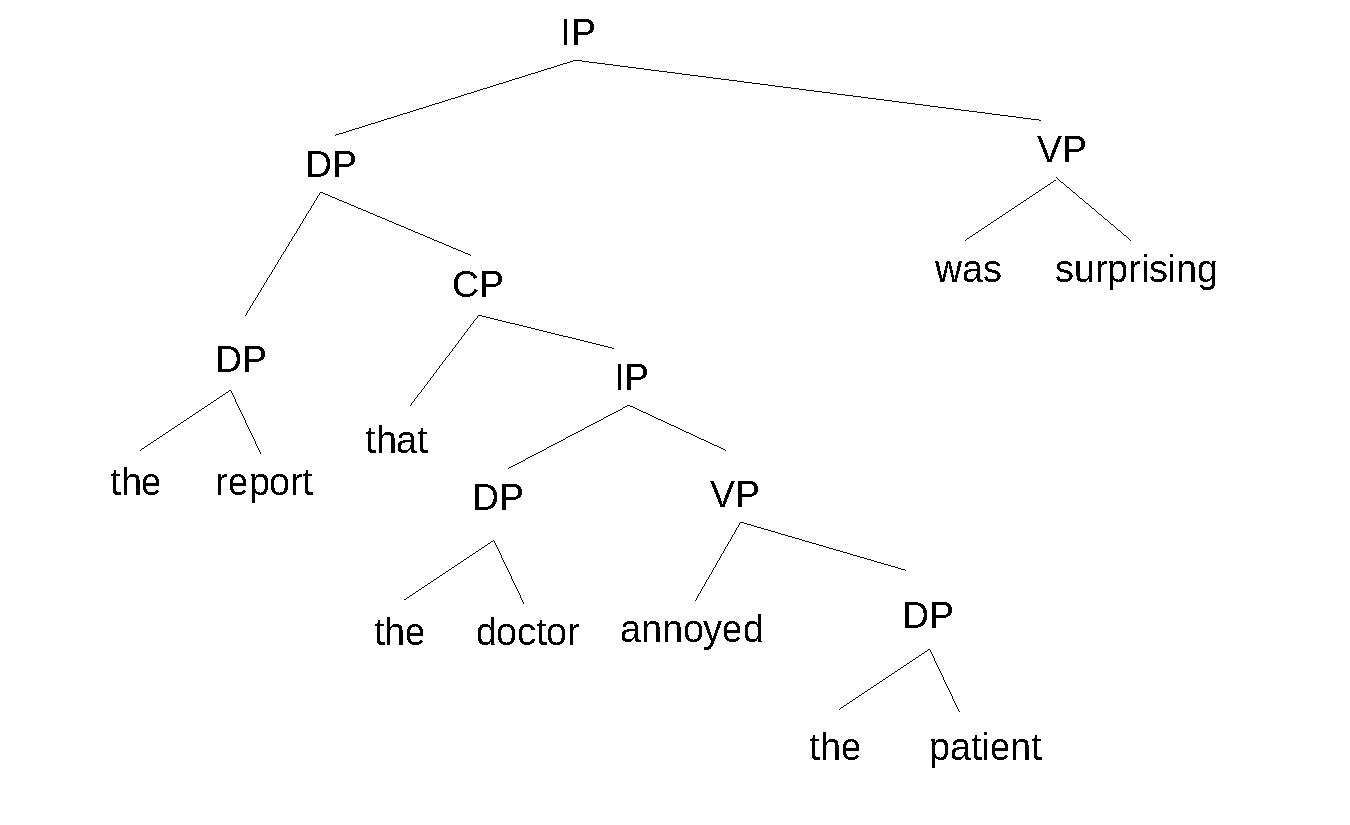
\includegraphics[width=0.5\textwidth]{figures/act-r-illustration-parsetree.pdf} \\
		(B) \\
		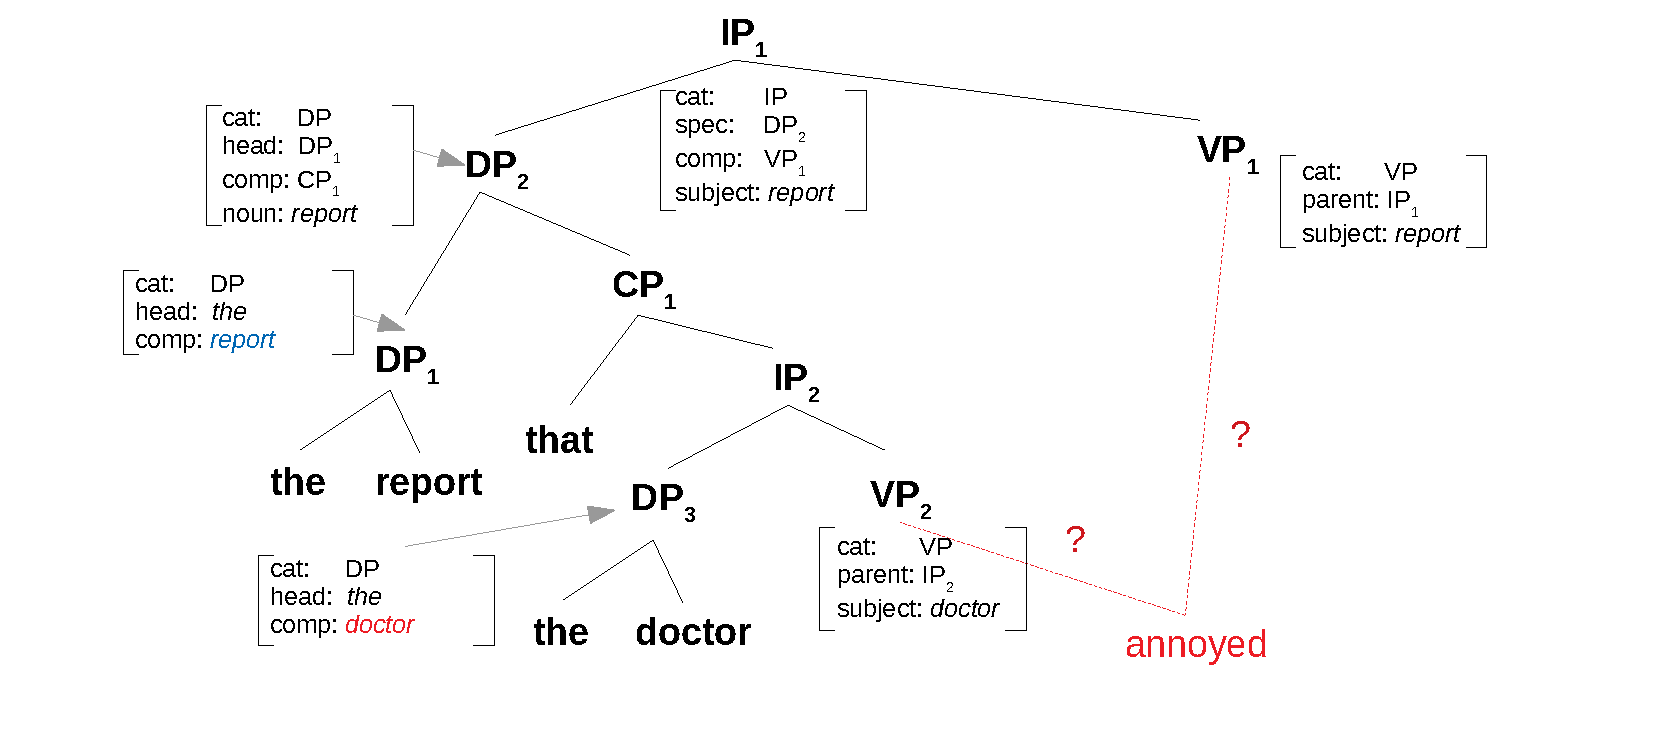
\includegraphics[width=0.5\textwidth]{figures/act-r-illustration-compatibility-cues.pdf} 
		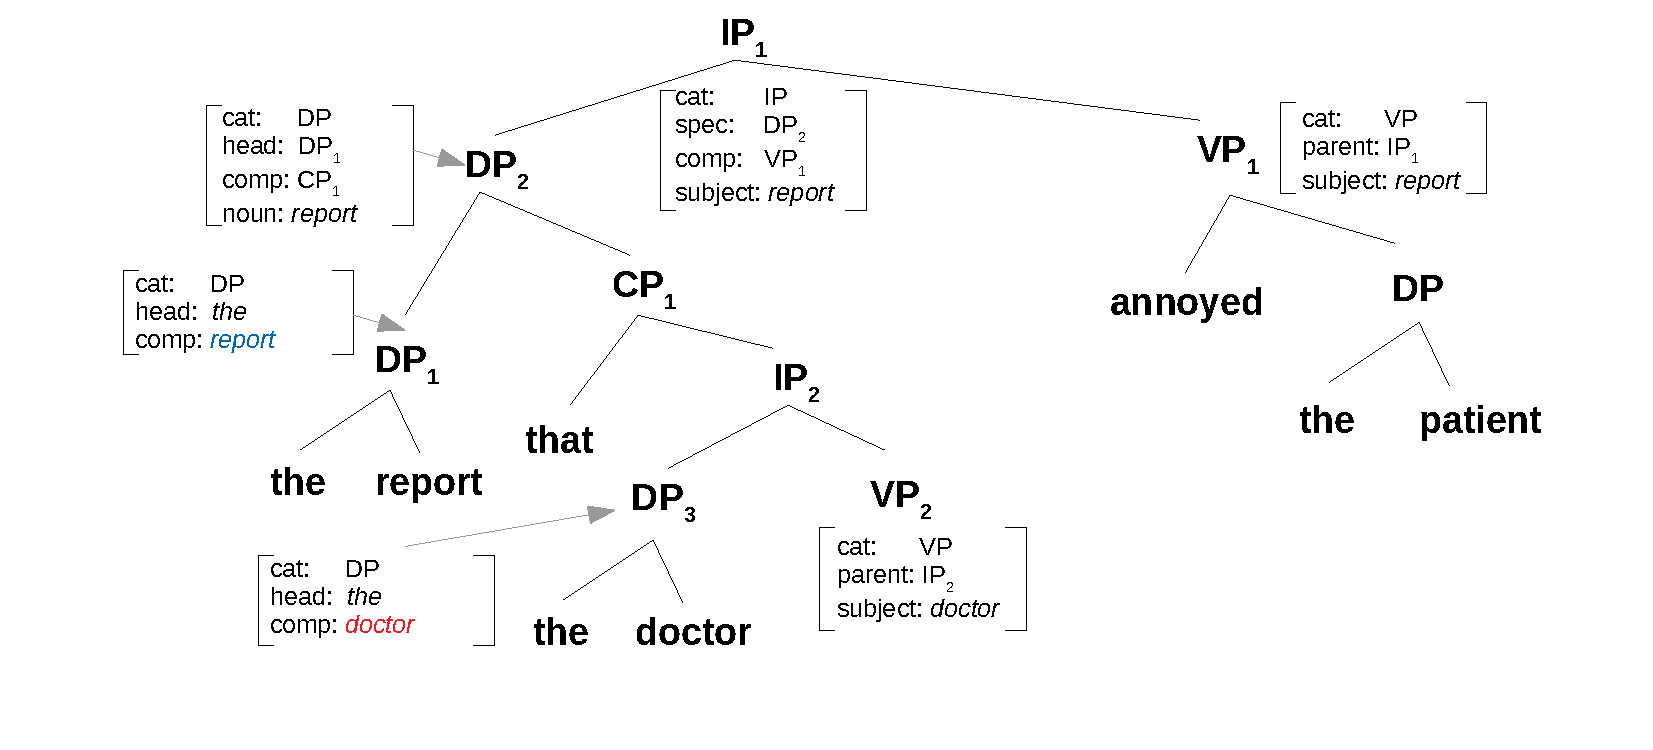
\includegraphics[width=0.5\textwidth]{figures/act-r-illustration-compatibility2-cues.pdf} 
	\end{tabular}
	\caption{Here, we sketch potential mechanisms by which a retrieval-based left-corner parser such as \citet{lewis2005activation} (similarly: \citet{Rasmussen2018LeftCornerPW, Dotlacil2020Parsing}) could be extended to produce the effect of semantic compatibility observed in our experiments. We note that, unlike Resource-Rational Lossy-Context Surprisal, the detailed predictions of such a retrieval-based parser crucially depend on specific assumptions about the grammar and parser rules; we here aim to illustrate what choices would be necessary to implement this effect. (A) Parse tree of a stimulus in the \textsc{Two} condition in the grammar formalism assumed by \citet{lewis2005activation}. (B) Left: Structure before ``annoyed'' is observed. Each node in the tree is described by a feature structure stored as a chunk in short-term memory. The current tree has two open predictions that both require a finite verb (at $VP_1$ and $VP_2$). Because the model does not represent serial order, it has to rely on other information to decide which of the two nodes to attach to. In this case, the two nodes are distinguished by their subject nouns (report and doctor); here, the model needs to assume that the parser percolates semantic information about the subject through the tree. As ``annoyed'' is semantically compatible with both subjects, semantic expectations do not rule out (incorrectly) attaching ``annoyed'' to $VP_1$. Right: Structure after completing this incorrect attachment. After completing $VP_1$, the top-level node $IP_1$ is marked as completed by the parser. Hence, the parser believes the sentence to be complete, leading to disruption when another verb is encountered.
	While such a mechanism could implement the effect of semantic compatibility, it is less clear how the retrieval-based parser could be extended to account for the effect of embedding bias, as it is not clear how the identity of the first noun impacts the choice of the attachment site for ``annoyed''. See text for further discussion.
	}
    \label{fig:retrieval}
\end{figure}



\subsection{Other Objective Functions}

We assumed that memory optimizations are optimized for next-word prediction.
Here, we compare to a model that instead assumes that representations are optimized to accurately represent the past, i.e., maximize the mutual information between the context $c$ and the representation $\representation$:
\begin{equation}\label{eq:objective-recovery}
	\min_\theta \mathbb{E}_{\contextInput^*w} \mathbb{E}_{\representation \sim p(\representation|\contextInput^*)} \left[- \log p(\contextInput|\representation)\right]
\end{equation}
where $p(\contextInput|\representation)$ is the posterior as displayed in Figure 2 in the main paper.
We solved this objective function using the same method as for our model, representing $p(\contextInput|\representation)$ using the inference network $q_\varphi(\contextInput|\representation)$ in formulating the variational Lagrangian objective function~(Equation \ref{eq:variational-lagrangian}).

Resulting model surprisal is shown in Figure~\ref{fig:model-surprisal-recovery}.
The model continues to qualitatively predict the three effects of interest: Surprisal is higher in \textsc{Three} than in \textsc{Two}, decreases with increased embedding bias in the \textsc{Two} and \textsc{Three} conditions, and is higher in  \textsc{Compatible} conditions than in \textsc{Incompatible} conditions.
The difference between \textsc{Two} and \textsc{Three} is reduced compared to the model optimizing for predictability, and compared to human reading times. We attribute this to the fact that the objective (\ref{eq:objective-recovery}) does not favor retaining recent elements more strongly, and therefore underpredicts locality effects.
While this locality effect is predicted by most theories of memory in sentence processing, the other two effects (embedding bias and compatibility in \textsc{Two}/\textsc{Three}) are not. It is therefore striking that the model (\ref{eq:objective-recovery}) strongly exhibits those, suggesting that they are quite robust to modeling assumptions within the broader framework combining Lossy-Contect Surprisal with resource-rational context representations.

\begin{figure}
    \centering

	\textbf{Experiment 1}
    

		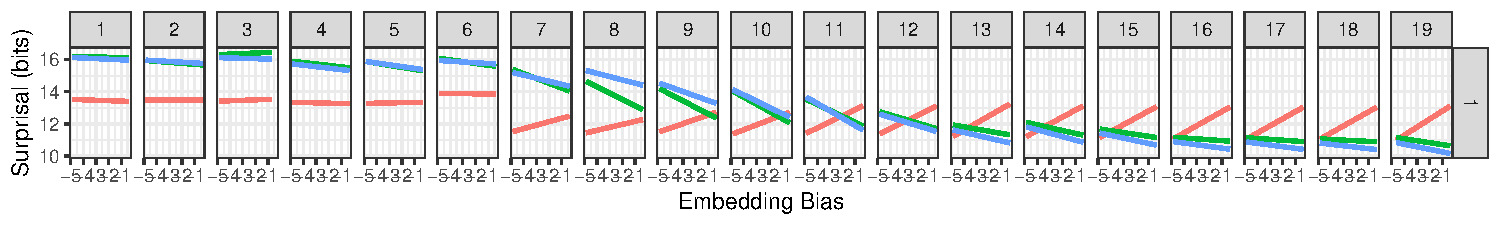
\includegraphics[width=0.8\textwidth]{../resource-rational-surprisal/model/compute_surprisal/analyze_output/figures/model-critical-experiment1-full-NoLimit_Lambda0_Integer_Bits.pdf} %&

	\textbf{Experiment 2}


    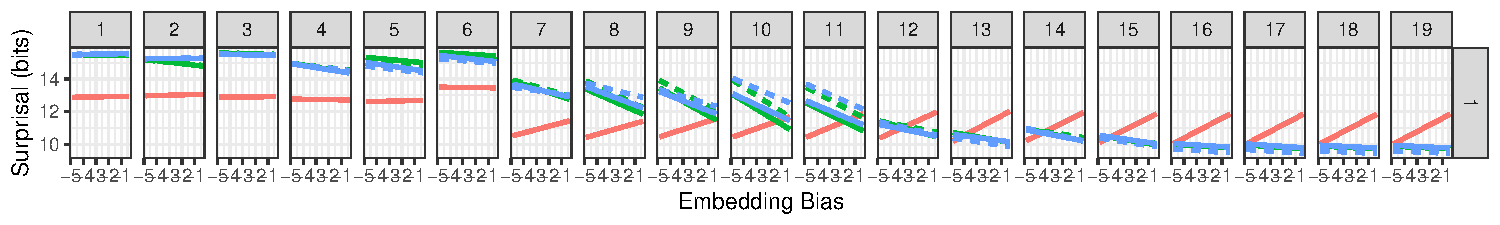
\includegraphics[width=0.8\textwidth]{../resource-rational-surprisal/model/compute_surprisal/analyze_output/figures/model-critical-experiment2-full-NoLimit_Lambda0_Integer_Bits.pdf}


        \begin{tabular}{llllllll}
\textbf{\textcolor{one}{----}} \textsc{One}&
\textbf{\textcolor{two}{----}} \textsc{Two}&
\textbf{\textcolor{three}{----}} \textsc{Three}
\end{tabular}
    
    \begin{tabular}{llllllll}
\textbf{{----}} \textsc{Incompatible}&
\textbf{{- - -}} \textsc{Compatible}
\end{tabular}
    
    
    
   
    \caption{Predictions for an alternative  model optimizing for recoverability of the context rather than next-word prediction: Model surprisal on the final verb across values of the retention rate $\deletionRate$. We show linear fits across all item-noun-pairs, averaged across all model runs at a given $\delta$.
	Compare Figure~\ref{fig:model-surprisal}.
	}
    \label{fig:model-surprisal-recovery}
\end{figure}


 


